\documentclass[../../dissertation.tex]{subfiles}
\begin{document}
In classical computation, a \textit{spatial search problem} focuses on finding marked points in a finite region of space. Defining this region with graphs is fairly straightforward, the vertices of the graph are the search space, and the edges define what transitions are possible through the search space. As was previously mentioned in \ref{chapGrover}, exhaustively searching through an unstructured space, by means of a classical random walk for example, would mean that in the worst case, one would have to take as many steps to find the marked points as there are vertices in the graph. Quantum computing provides an alternative to this complexity through Grover's algorithm, and applying some of his ideas to the coined quantum walk not only allows a quantum counterpart to the random walk search, but also further insight into the algorithm itself.\par
%TODO:\textcolor{red}{acho que você precisa delimitar o que fará ao longo desta seção, dizer que tratará os três modelos e a busca}
Following \cite{REN1}'s definition, a good first step is to borrow the diffusion from Grover's algorithm and invert the sign of the state corresponding to the marked vertex while leaving unmarked vertices unchanged. This is done through the following operator 
%TODO:\textcolor{red}{eu trocaria a notação de $\mOathcal{F}$ por $\mathcal{O}$ e dizer que é um oráculo}
\begin{equation}
	\mathcal{O} = I - 2 \sum_{x\in M} \ket{x}\bra{x}
\end{equation}
where M is the set of marked vertices and $\mathcal{O}$ is an analogue to Grover's oracle. For one marked vertex, this oracle can be written as 
%TODO:\textcolor{red}{você pode até dizer que $M=\{0\}$}
\begin{equation}
	\mathcal{O} = I - 2 \ket{0}\bra{0}
\end{equation}
Notice that there is no loss of generality by choosing the marked vertex as $0$, since the labelling of the vertices is arbitrary.\par
The next step is to combine the evolution operator from the coined quantum walk model with the oracle
\begin{equation}
	U'= U\mathcal{O}
	\label{eq:43}
\end{equation}
Similarly to the simple coined case, the walker starts at $\ket{\Psi(0)}$ and evolves following the rules of an unitary operator $U$ followed by the sign inversion of marked vertices. The walker's state after an arbitrary number of steps will be
\begin{equation}
	\Psi(t) = (U')^t\ket{\Psi(0)}.
	\label{eq:sysStateSearch}
\end{equation}\par

For a better understanding of the search problem in the coined quantum walk model, consider a graph where all the vertices are connected and each vertex has a loop that allows transitions to itself, as shown in figure \ref{fig:undCompGraph}. 
%TODO: \textcolor{red}{não precisa dizer que são arcos também}
%                \begin{figure}[!h]
%                \centering
%                \begin{tikzpicture}[shorten >=1pt,auto,node distance=3cm,
%                    thick,main node/.style={circle,draw,font=\sffamily\Large\bfseries}]
%
%                      \node[main node] (1) {1};
%                      \node[main node] (2) [below left of=1] {2};
%                      \node[main node] (3) [below right of=2] {3};
%                      \node[main node] (4) [below right of=1] {4};
%                    
%                      \path[every node/.style={font=\sffamily\small}]
%                        (1) edge node [left] {} (4)
%                            edge [loop above] node {} (1)
%                            edge node [below] {} (3)
%                        (2) edge node [right] {} (1)
%                            edge node {} (4)
%                            edge [loop left] node {} (2)
%                        (3) edge node [right] {} (2)
%                            edge [loop below] node {} (3)
%                        (4) edge node [left] {} (3)
%                            edge [loop right] node {} (4)
%                 \end{tikzpicture}
%                  \caption{Undirected Complete Graph}
%                  \label{fig:undCompGraph}
%                \end{figure}
%                \textcolor{red}{acho que não há necessidade das figuras e dizer que é com grafo direcionado}
%                Grover's algorithm is equivalent to a coined quantum walk on a directed complete graph with loops such as the one in figure \ref{fig:dirCompGraph}.
%                \begin{figure}[!h]
%                    \centering
%                    \begin{tikzpicture}[->,>=stealth',shorten >=1pt,auto,node distance=3cm,
%                    thick,main node/.style={circle,draw,font=\sffamily\Large\bfseries}]
%                      \node[main node] (1) {1};
%                      \node[main node] (2) [below left of=1] {2};
%                      \node[main node] (3) [below right of=2] {3};
%                      \node[main node] (4) [below right of=1] {4};
%                      \path[every node/.style={font=\sffamily\small}]
%                        (1) edge node [bend left] {} (4)
%                            edge [bend right] node[left] {} (2)
%                            edge [loop above] node {} (1)
%                            edge node [arc below] {} (3)
%                        (2) edge node [bend right] {} (1)
%                            edge node {} (4)
%                            edge [loop left] node {} (2)
%                            edge [bend right] node[left] {} (3)
%                        (3) edge node [right] {} (2)
%                            edge [bend right] node[right] {} (4)
%                            edge node [bend up] {} (1)
%                        (4) edge node [left] {} (3)
%                            edge [loop right] node {} (4)
%                            edge [bend right] node[right] {} (1)
%                            edge node [bend left] {} (2);
%                    \end{tikzpicture}
%                    \caption{Directed complete graph with N=4 nodes.}
%                    \label{fig:dirCompGraph}
%                \end{figure}    
%                
The next step is to label the arcs using notation $\{(v,v'), v \geqslant 0 \land v' \leqslant N-1\}$ 
where $N$ is the total number of vertices and $(v,v')$ are the position and coin value, respectively, in the coined model. 
%sera que vale a pena desenhar um grafo com labels?
The shift operator, now called \textit{flip-flop} shift operator, is
\begin{equation}
	S\ket{v1}\ket{v2} = \ket{v2}\ket{v1}.
	\label{eq:chap3FlipFlop}
\end{equation}\par
The coin operator is defined as
\begin{equation}
	C = I_N \otimes G
\end{equation}
where 
%TODO:\textcolor{red}{prefiro s a D}
\begin{equation}
	G = 2\ket{D}\bra{D} - I
\end{equation}
is the Grover coin with $\ket{D}$ being the diagonal state of the coin space. Given both of these operators, the evolution is defined for the unmarked case similarly to \ref{coinedUnmarkedOperator}
\begin{equation}
	U = S(I \otimes G).
\end{equation}\par
Marking an element in a complete graph is done through the following oracle
\begin{equation}
	\mathcal{O'} =\mathcal{O}\otimes I = (I_N - 2\ket{0}\bra{0})\otimes I_N = I_{N^2} - 2 \sum_v \ket{0}\ket{v}\bra{0}\bra{v} ,
\end{equation}
that can be seen, in the arc notation, as an operator that marks all arcs leaving $0$.\par
Recalling \ref{eq:43}, the modified evolution operator can be written as
\begin{equation}
	U' = S(I \otimes G)\mathcal{O'} = S(I \otimes G)\mathcal{O} \otimes I = S (\mathcal{O} \otimes G),\label{eq:modifiedEvoCoined}
\end{equation}
and the state of the system will evolve according to equation \ref{eq:sysStateSearch}.\par
As was shown in \cite{REN1}, maximum probability of the marked vertex is achieved after $\frac{\pi}{2}\sqrt{N}$ steps. Figure \ref{fig:coinedSearch} is the result of coding and plotting the evolution of this probability distribution, for graphs of varying sizes. It shows that the probability is close to one at \textit{approximately} the predicted ideal steps, because of the discrete nature of the walk. The probability distributions have a stair-like shape, because transitions in this model only occur on even numbered time steps, because of how the unmodified evolution operator was constructed.

\begin{figure}[!h]
	\centering
	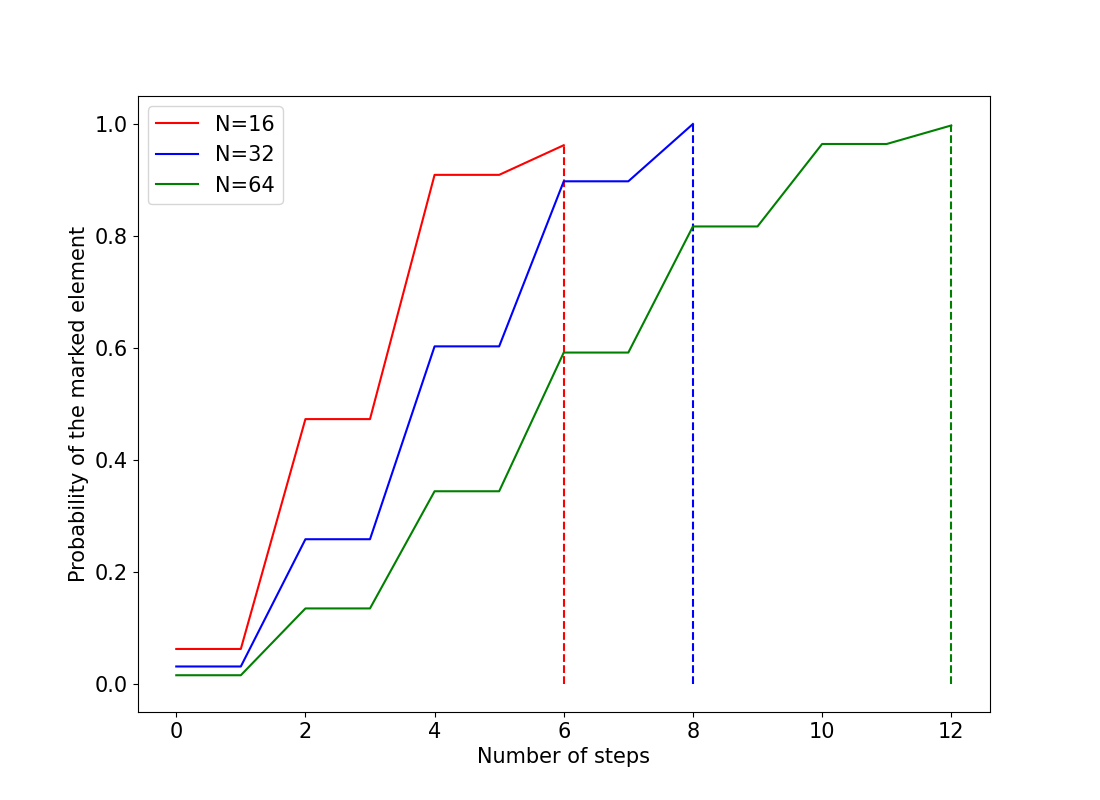
\includegraphics[scale=0.40]{img/CoinedQuantumWalk/Search/CoinedSearch163264.png}
	\caption{Discrete-time coined quantum walk search for a complete graph with 16, 32 and 64 nodes.}\label{fig:coinedSearch}
\end{figure}

\end{document}
